%% Copyright (c) 2004  SciSoft.  All rights reserved.
%%
%% This file is part of CGAL (www.cgal.org); you may redistribute it under
%% the terms of the Q Public License version 1.0.
%% See the file LICENSE.QPL distributed with CGAL.
%%
%% Licensees holding a valid commercial license may use this file in
%% accordance with the commercial license agreement provided with the software.
%%
%% This file is provided AS IS with NO WARRANTY OF ANY KIND, INCLUDING THE
%% WARRANTY OF DESIGN, MERCHANTABILITY AND FITNESS FOR A PARTICULAR PURPOSE.
%%
%% 
%%
%% Author(s)     : Fernando Cacciola <fernando_cacciola@hotmail.com>





\begin{figure}[htbp]
\begin{ccTexOnly}
\begin{center}
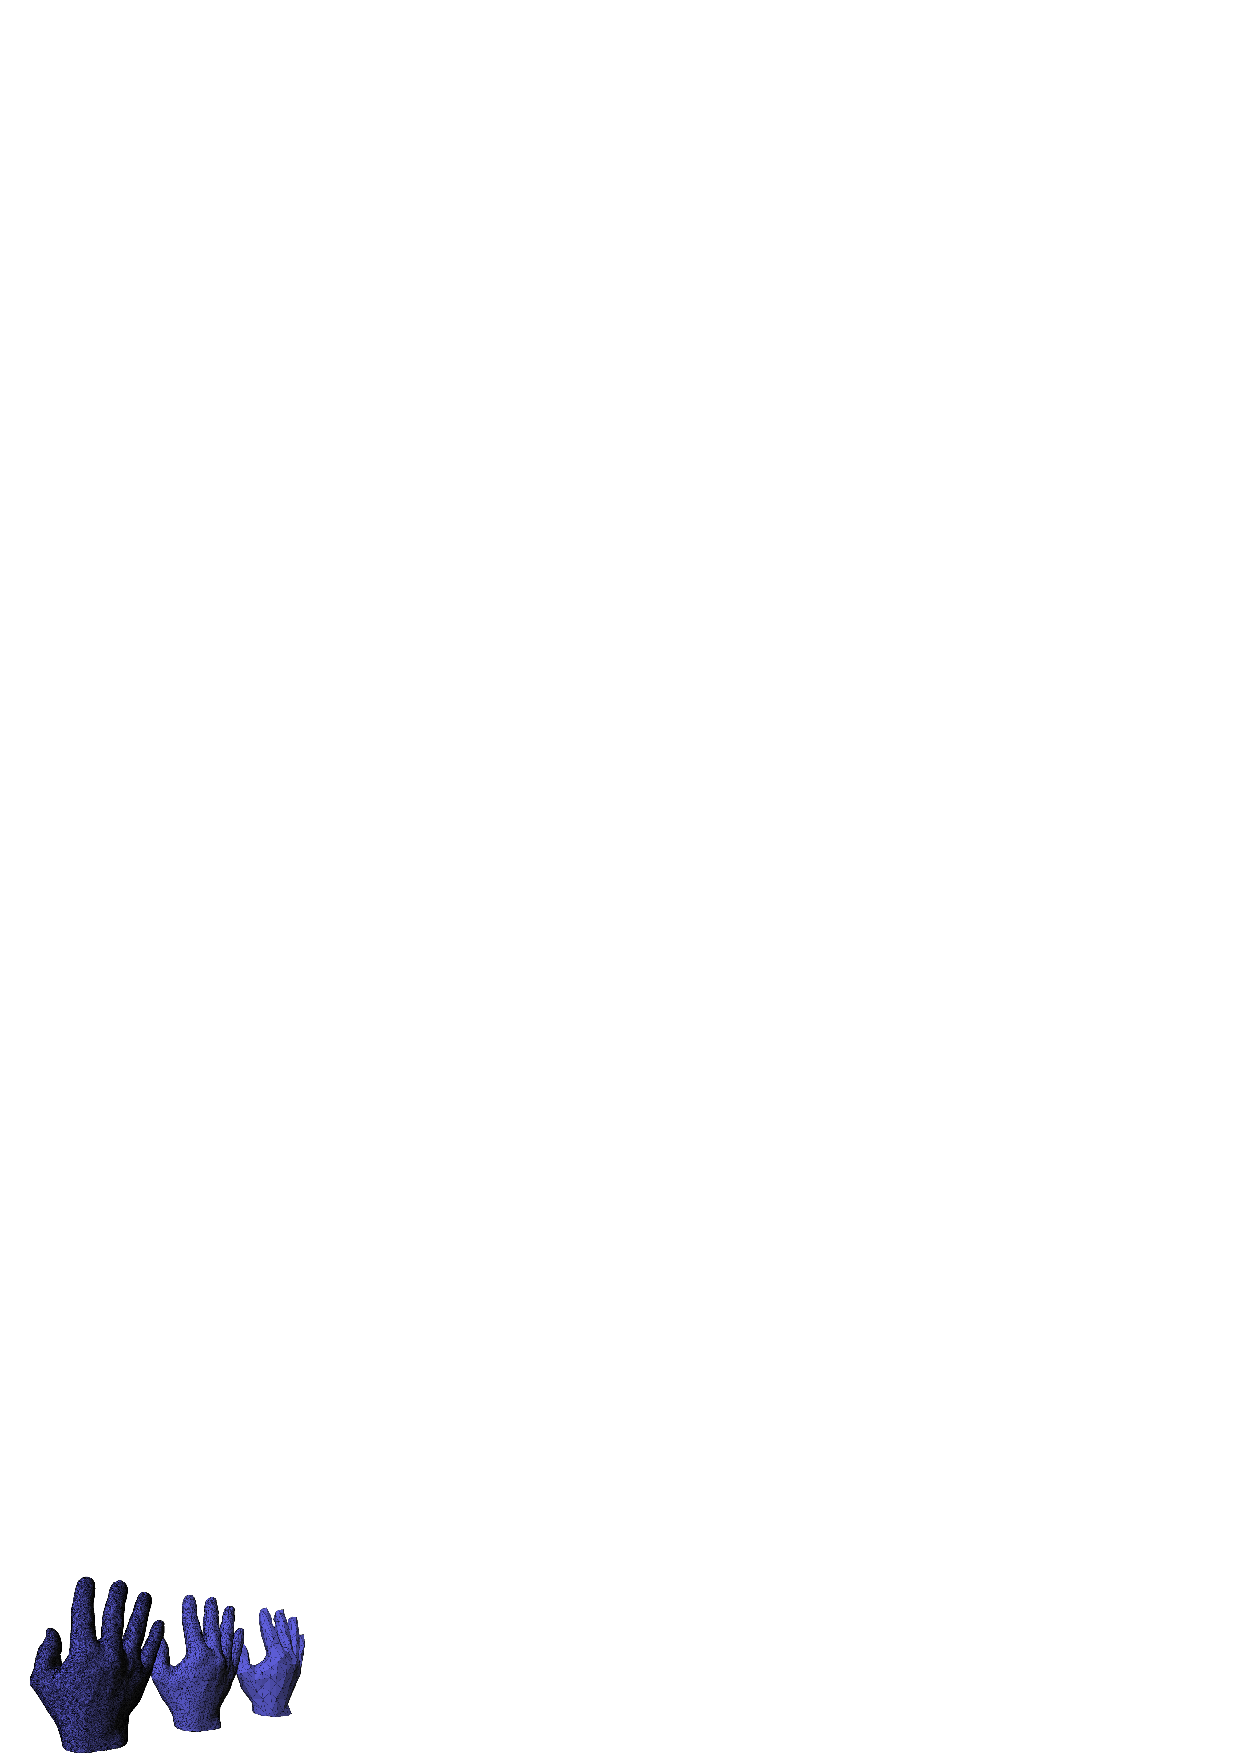
\includegraphics[width=17cm]{Surface_mesh_simplification/fig/Illustration-Simplification-ALL} % omit suffix .eps to support PS and PDF
\end{center}
\end{ccTexOnly}
\begin{ccHtmlOnly}
<TABLE CELLSPACING=40>
<TR>
<CENTER>
<IMG BORDER=0 SRC="./fig/Illustration-Simplification-ALL.png" ALIGN=center ALT="Simplification illustration">
</CENTER>
</TR>
</TABLE>
\end{ccHtmlOnly}
\end{figure}
%% figures of simplified surfaces

\section{Introduction}
Surface mesh  simplification is the process of reducing the number of faces used in the surface while 
keeping the overall shape, volume and boundaries preserved as much as possible. 
It is the opposite of subdivision.

The algorithm presented here can simplify any {\em open oriented 2-manifold surface},
with any number of connected components, with or without boundaries (border or holes) 
and handles (arbitrary genus), using a method known as {\em edge collapse}.
Roughly speaking, the method consists of iteratively replacing an edge with a single vertex, 
removing 2 triangles per collapse.

%% figure of edge collapse

Edges are collapsed according to a priority given by a user-supplied {\em cost} function,
and the coordinates of the replacing vertex are determined by another user-supplied
{\em placement} function. The algorithm terminates when a user-supplied {\em stop predicate} 
is met, such as reaching the desired number of edges.

The algorithm implemented here is generic in the sense that it does not require the surface 
to be of a particular type. Instead, it defines the concept of a \ccc{EdgeCollapsableMesh}
and any surface that is a model of that concept can be simplified. Furthermore, the concept
is defined not in terms of a monolithic class, but in terms of a set of functions and traits,
making it easy to adapt any concrete surface type. In particular, the concept definition 
follows the design of the 
\ccAnchor{http://www.boost.org/libs/graph/doc/index.html}{ Boost Graph Library ({\sc Bgl})}.

The design is \ccAnchor{http://en.wikipedia.org/wiki/Policy-based_design}{{\em policy-based}},
meaning that you can customize some aspects of the process by passing a set of
{\em policy objects}. Each policy object specifies a particular aspect of the algorithm,
such as how edges are selected and where the replacement vertex is placed. All policies have 
a sensible default.
Furthermore, the API uses the so-called \ccc{named-parameters} technique which allows you
to pass only the relevant parameters, in any order, omitting those parameters whose
default is appropriate.

\section{Overview of the Simplification Process}

The free function that implements the simplification algorithm takes not only the surface
and the desired stop predicate but a number of additional parameters which control and
monitor the simplification process. This section briefly describes the process in order 
to set the background for the discussion of algorithm parameters.

An edge collapse operation replaces the edge with a vertex, removing the two incident 
triangles (hence two additional edges, one from each triangle). Therefore, each edge collapse 
decreases the number of triangles, edges, and vertices by 2, 3, and 1, respectively 
(if the collapsed edge is a border, by 1,2, and 1, respectively, since only one triangle 
is removed).

Naturally, the surface that results from an edge collapse deviates from the initial 
surface by some amount, and since the goal of simplification is to reduce the number 
of triangles while retaining the overall look of the surface as much as possible, 
it is necessary to measure such a deviation. Some methods attempt to measure the 
total deviation from the initial surface to the completely simplified surface, 
for example, by tracking an accumulated error while keeping a history of the simplification 
changes. Other methods, like the one implemented in this package, attempt to measure only
a step {\em cost} (the local deviation introduced by a single simplification step) and 
plan the entire process as a sequence of steps of increasing cost. 

Global error tracking methods produce highly accurate simplifications but take up a lot 
of additional space. Cost-driven methods, like the one in this package, produce slightly 
less accurate simplifications but take up much less additional space, even none in some cases.

The cost-driven method implemented in this package is mainly based on \cite{cgal:lt-fmeps-98,cgal:lt-ems-99}, with contributions from \cite{hddms-mo-93}, \cite{gh-ssqem-97}
and \cite{degn-tpec-98}.

The algorithm proceeds in two stages. In the first stage, called {\em collection stage}, 
an initial {\em collapse cost} is assigned to each and every edge in the surface.
Then in the second stage, called {\em collapsing stage}, edges are 
processed in order of increasing cost. Some processed edges are collapsed 
while some are just discarded. Collapsed edges are replaced by a vertex and the collapse 
cost of all the edges now incident on the replacement vertex is recalculated, affecting 
the order of the edges left to process.

Not all edges selected for processing are collapsed. A processed edge can be discarded 
without being collapsed for one of three reasons: its cost could not be computed 
(for whatever reason), collapsing the edge would result in an inconsistent surface, 
or the edge is incident upon a vertex which the user marked as fixed.

If an edge is effectively collapsed, it is replaced by a vertex whose position, called 
{\em placement}, is chosen carefully to avoid too much deviation from the initial 
surface. In many cases, the collapse cost is a function of the vertex position, so the 
placement might be calculated each time the cost is calculated and not just when an 
edge is effectively collapsed.

The algorithm presented in \cite{gh-ssqem-97} collapses arbitrary vertex pairs and not 
only edges by considering certain vertices as forming a pseudo-edge, proceeding to collapse
both edges and pseudo-edges in the same way as in \cite{cgal:lt-fmeps-98,cgal:lt-ems-99}, 
which is the algorithm implemented here. Since it is always possible to physically add and 
remove those pseudo-edges (and the required pseudo-triangles needed to keep the surface 
structurally valid), this \cgal\ package can be used to implement the algorithm
in \cite{gh-ssqem-97} if the appropriate cost-strategy policies are added 
(they are not implemented in the current version) and a pre/post processing phase that
adds and removes pseudo-edges is used.

\section{Cost Strategy}

The specific way in which the collapse cost and vertex placement is
calculated is called the {\em cost strategy}. The user can choose 
different strategies in the form of policies and related parameters,
passed to the algorithm.
 
The current version of the package provides a set of policies implementing
two strategies: the Lindstrom-Turk strategy, which is the default, and 
a strategy consisting of an edge-length cost with a midpoint placement 
(much faster but less accurate).

\subsection{Lindstrom-Turk Cost and Placement Strategy\label{SurfaceMeshSimplification:LindstromTurkStrategy}}

The main characteristic of the strategy presented in
\cite{cgal:lt-fmeps-98,cgal:lt-ems-99} is that the simplified surface
is not compared at each step with the original surface (or the surface
at a previous step) so there is no need to keep extra information,
such as the original surface or a history of the local changes. Hence
the name {\em memoryless} simplification.

At each step, all remaining edges are potential candidates for a
collapsing and the one with the lowest cost is selected.

The cost of collapsing an edge is given by the position chosen for the
vertex that replaces it. From all the potential vertex positions, the
one that minimizes the local change in each of the relevant surface
features (volume, area, boundary shape and triangles shape) is
chosen. The cost is then a weighted sum of that minimal change in each
of the relevant features.

 The local changes are computed independently for each edge using only
the triangles currently adjacent to it, after all previous
collapses, so the transitive path of minimal local changes yields at
the end a global change reasonably close to the absolute minimum.

\subsection{Cache Level}

The cost for each edge is initially fixed and changes only in those edges 
affected by a neighboring collapse. A given edge can be expected to be 
affected by a neighboring collapse only a small number of times 
(in the order of the average vertex degree), so the total number of 
cost computations and recomputations is a small factor of
the total number of edges. 
On the other hand, edges are processed in order of increasing cost, and as is 
the case with any sorting situation, the cost of any given edge must be accessed 
several times while it is compared against the cost of other edges, even if it 
remains constant. That is, costs are queried several times more than are computed 
and updated, so it make sense to cache the cost of an edge to avoid recomputing it.

The placement for each edge is queried only when the edge is effectively collapsed. 
However, most cost strategies are based on the placement so each cost computation 
typically involves a hidden placement computation. Therefore, it might also make sense
to cache not only the cost but also the placement (which is a \ccc{Point} object).

Caching only the cost as opposed to caching both the cost and the placement makes a
small fractional difference in the total running time because the cost for the
edges is computed at least once and updated a few times (on average), while the 
placement is queried only when the edge is effectively collapsed. Not caching 
anything, on the other hand, causes a significant slowdown because the cost is
unnecessarily recomputed each time one candidate edge is compared with another.

Still, caching the cost and/or placement in the edge adds to the size of the surface 
a significant amount. For example, if the cost is of type {\tt double} and a vertex
position is a 3D point with {\tt double} coordinates, each million edges require 
about 7Mb of additional storage for the cost, and 30Mb for the cost and placement.
For certain applications, it might be better to avoid any caching altogether, even 
at the expense of increased running time.
 
By default, only the cost is cached, which is the most sensible tradeoff.

\subsection{Cost Strategy Policies}

The cost strategy used by the algorithm is selected by means of three policies: 
\ccc{SetCache}, \ccc{GetCost} and \ccc{GetPlacement}. 

The \ccc{SetCache} policy controls whether the cache is empty (\ccc{NoCache}), 
stores the cost but not the placement(\ccc{CostCache}), or stores both 
(\ccc{CostAndPlacementCache)}.

The \ccc{GetCost} and \ccc{GetPlacement} policies are called each time
the algorithm needs to access the cost or placement for an edge.
If an empty cache is used, these functions must effectively
calculate the values and return it, but otherwise they can 
(and normally would) simply return the cached value.

If \ccc{SetCache} actually stores any value in the cache, it computes
such a value by calling itself a GetCost and/or GetPlacement
policy (other than the ones passed to the algorithm).

The three policies are related in that if \ccc{SetCache}
assigns a \ccc{NoCache} record, the \ccc{GetCost} and \ccc{GetPlacement} policies
must be actually computing the values, while if \ccc{SetCache} sets a 
\ccc{CostCache}, only \ccc{GetPlacement} would actually compute a value since
\ccc{GetCost} would simply return the cached cost.
Similarly, if \ccc{SetCache} assigns a \ccc{CostAndPlacementCache} record, 
the other two policies would just return the cached values.

\section{API}

\subsection{API Overview}

The simplification algorithm is implemented as the free template function 
\ccc{CGAL::Surface_mesh_simplification::edge_collapse}. THe function has two mandatory and several optional parameters.

\begin{cprog}
int r = edge_collapse(surface,
                     stop_predicate,
                     
                     vertex_point_map   (vertex_point_map_arg)
                     .edge_index_map     (edge_index_map_arg)
                     .edge_is_border_map (edge_is_border_map_arg)
                     .vertex_is_fixed_map(vertex_is_fixed_map_arg)
                     
                     .set_cache          (set_cache_arg)
                     .get_cost           (get_cost_arg)
                     .get_placement      (get_placement_arg)
                     .cost_params        (cost_params_arg)
                     .placement_params   (placement_params_arg)
                     
                     .visitor            (visitor_arg)
                     );
\end{cprog}

\subsubsection{Mandatory Parameters}

There are two main parameters to the algorithm: the surface to be simplified (in-place) and the stop predicate.

The surface to simplify must be a model of the \ccc{EdgeCollapsableMesh} concept. 
Many concrete surface types, such as \ccc{CGAL::Polyhedron_3}, become models of 
that concept via a technique known as 
{\em external adaptation} 
(see \ccAnchor{http://www.boost.org/libs/graph/doc/leda_conversion.html}
{this {\sc Bgl} page for details}). External adaptation is a way to add an interface to an 
object without coercing the type of the object (which happens when you adapt it by means 
of a wrapper). That is, the formal parameter to the \ccc{edge_collapse} function that 
implements the simplification is the concrete surface object itself, not an adaptor 
which delegates the functionality to the concrete type.

The stop predicate is called after each edge is selected for processing, {\em before} 
it is classified as collapsable or not (thus before it is collapsed). If the stop predicate 
returns \ccc{true} the algorithm terminates.

\subsubsection{Optional Named Parameters}

The notion of {\em named parameters}, was introduced with the
\ccAnchor{http://www.boost.org/libs/graph/doc/bgl_named_params.html}{{\sc Bgl} algorithms}.
Thay allow the user to specify only those parameters which are really needed,
and they are specified by name, making the parameter ordering unimportant. 

One of the named parameters is a visitor object which can be used to track the simplification 
process. Some of the named parameters are property maps which supply information about 
the surface, and the rest correspond to the cost-strategy policies. 

Note that the list of named parameters is really a composition
of function calls separated by a dot ($.$). Any of these named parameters can be omitted, 
and they can be in any order.



\subsection{Examples}

The following examples introduce the API in increasing complexity. All the examples follow 
this general structure:

\ccIncludeExampleCode{Surface_mesh_simplification/general_form.cpp}

Each example varies from this general form in the code sections between 
the marks. As the examples are compilable some necessary parts are repeated 
in many of them. To simplify the exposition, repeated parts are described in detail 
only in the first example they appear.

\subsubsection{Example Using Default Parameters}

The following example illustrates the simplest of the cases. It uses
an ordinary polyhedron, that is, a polyhedron without any special
provision for the sake of the algorithm (which is possible as
illustrated in the next example).  Many parameters are omitted,
causing the algorithm to run in default mode:

\begin{itemize}
\item There are no fixed vertices in the surface.
\item The cost strategy is that of Lindstrom-Turk, computed with default parameters 
      and caching only the cost.
\item No visitor is used to track the algorithm progress.
\end{itemize}

\ccIncludeExampleCode{Surface_mesh_simplification/LT_edge_collapse_polyhedron.cpp}

\subsubsection{Example Using Enriched Polyhedron}

The following example is equivalent to the previous example but using an
enriched polyhedron whose halfedges support an \ccc{id} field to
store the edge index needed by the algorithm.

\ccIncludeExampleCode{Surface_mesh_simplification/LT_edge_collapse_enriched_polyhedron.cpp}

\subsubsection{Example using Non-Default Cost Strategy}

The following example shows how to use a non-default cost strategy: the edge squared length
as cost and the edge midpoint as placement. This strategy is less accurate but
is very fast so there is little need for a cache. The example shows how to specify 
that neither the cost nor the placement should be cached, saving memory.

\ccIncludeExampleCode{Surface_mesh_simplification/MP_edge_collapse_polyhedron.cpp}

\subsubsection{Example Using a Full Cost and Placement Cache}

The following example shows how to use a full cache for maximizing speed.
The required code for the default cost-strategy (Lindstrom-Turk) is
slightly different than the code needed for alternative strategies,
so both cases are shown.

\ccIncludeExampleCode{Surface_mesh_simplification/Edge_collapse_fully_cached_polyhedron.cpp}

\subsubsection{Example using a Visitor}

The following example shows how to use a visitor to track the simplification process. 
It also shows how to setup the Lindstrom-Turk cost strategy but with a cost-only 
cache (unlike a full cache as in the previous example). A cost-only cache is
the default policy so you don't really need to explicitly specify it. It is shown here
for illustration.

\ccIncludeExampleCode{Surface_mesh_simplification/LT_edge_collapse_visited_polyhedron.cpp}


\subsubsection{Example using Fixed Vertices via an External Map}

The following example shows how to fix vertices to prevent edges from being collapsed. 
In this case, an ordinary polyhedron is used and the flags are stored 
in an external hashmap.

\ccIncludeExampleCode{Surface_mesh_simplification/LT_edge_collapse_with_fixed_vertices_polyhedron.cpp}

\subsubsection{Example using Fixed Vertices via an Enriched Polyhedron}

The following example, just like the previous example, shows how to fix vertices to 
prevent edges from being collapsed. In this case, however, an enriched polyhedron 
is defined which stores the flag right in the vertex.

\ccIncludeExampleCode{Surface_mesh_simplification/LT_edge_collapse_with_fixed_vertices_enriched_polyhedron.cpp}

% +------------------------------------------------------------------------+
%%RefPage: end of main body, begin of sfsooter
% EOF
% +------------------------------------------------------------------------+


